\documentclass[12pt]{article}
        \makeatletter
        \def\input@path{{../../}}
        \makeatother
        \usepackage{sbc-template}
        \makeatletter
        \renewcommand{\inst}[1]{}
        \makeatother
        \usepackage{graphicx,url}
        \usepackage[utf8]{inputenc}
        \usepackage[T1]{fontenc}
        \usepackage[brazil]{babel}
        \usepackage{longtable,booktabs,array}
        \usepackage{amsmath,amssymb}
        \providecommand{\tightlist}{%%
          \setlength{\itemsep}{0pt}\setlength{\parskip}{0pt}}
        \sloppy
        \title{De Reservoir Computing classico a Quantum Reservoir Computing: a ponte conceitual}
        \author{}
        \address{}
        \begin{document}

        \maketitle

        \begin{resumo}
        Este artigo constroi a ponte entre o RC classico estudado ate aqui e o QRC usado no estudo final. O objetivo e mostrar que QRC nao nasce como um tema separado do restante da obra, mas como uma extensao natural da ideia de reservatorio: manter a separacao entre dinamica rica e readout simples, trocando o meio classico por um meio quantico. O texto apresenta o paralelo formal entre RC e QRC, mapeia essa ponte para a implementacao em Qiskit, discute a estrategia de tuning usada no projeto e introduz a funcao objetivo que equilibra desempenho e complexidade (\texttt{qubits}, \texttt{window}). Ao final, o leitor sabe por que duas configuracoes candidatas emergiram do tuning: \texttt{14x7} como melhor ponto multi-metrica e \texttt{8x5} como melhor compromisso segundo a funcao objetivo escalar.
        \end{resumo}

        \subsection{1. O que o leitor vai aprender}\label{1-o-que-o-leitor-vai-aprender}

Ao final deste artigo, voce sera capaz de:

\begin{enumerate}
\def\labelenumi{\arabic{enumi}.}
\tightlist
\item
  enxergar RC e QRC dentro do mesmo paradigma;
\item
  entender como entradas classicas sao codificadas em circuitos quanticos;
\item
  ler a implementacao do QRC em \texttt{code/qrc/model.py};
\item
  interpretar o tuning de \texttt{n\_qubits} e \texttt{window};
\item
  justificar tecnicamente por que \texttt{14x7} e \texttt{8x5} foram preservados para o artigo final.
\end{enumerate}

\subsection{2. RC como paradigma geral}\label{2-rc-como-paradigma-geral}

No RC classico, a ideia e:

\[
u_t \longrightarrow x_t \longrightarrow \phi_t \longrightarrow \hat{y}_t.
\]

Em outras palavras:

\begin{itemize}
\tightlist
\item
  a entrada \(u_t\) perturba um sistema dinamico;
\item
  o sistema responde com um estado \(x_t\);
\item
  o readout linear aprende a ler esse estado.
\end{itemize}

O QRC preserva exatamente essa logica. O que muda e o meio em que a dinamica interna acontece.

\subsection{3. O salto para o quantico}\label{3-o-salto-para-o-quantico}

No projeto, o reservatorio quantico usa circuitos de reuploading implementados com Qiskit. Para cada qubit \(q\) e para cada passo de entrada, a codificacao usa angulos do tipo

\[
\theta^{(q,t)}_x = s \, w_{x,q}^\top u_t + b_q,
\qquad
\theta^{(q,t)}_y = s \, w_{y,q}^\top u_t,
\]

em que:

\begin{itemize}
\tightlist
\item
  \(u_t \in \mathbb{R}^4\) e o vetor classico reduzido;
\item
  \(s\) e \texttt{input\_scale};
\item
  \(w_{x,q}\) e \(w_{y,q}\) sao pesos aleatorios por qubit.
\end{itemize}

O circuito elementar do projeto aplica:

\begin{enumerate}
\def\labelenumi{\arabic{enumi}.}
\tightlist
\item
  \texttt{RX} e \texttt{RY} em cada qubit;
\item
  um anel de emaranhamento \texttt{CZ};
\item
  rotacoes \texttt{RZ} apos cada acoplamento.
\end{enumerate}

\subsection{4. Paralelo direto entre RC e QRC}\label{4-paralelo-direto-entre-rc-e-qrc}

O paralelo conceitual entre os dois modelos pode ser escrito assim:

\begin{longtable}[]{@{}ll@{}}
\toprule\noalign{}
RC classico & QRC do projeto \\
\midrule\noalign{}
\endhead
\bottomrule\noalign{}
\endlastfoot
estado vetorial \(x_t\) & estado quantico \$ \\
matriz recorrente \(W_{res}\) & circuito com \texttt{RX}, \texttt{RY}, \texttt{CZ}, \texttt{RZ} \\
features \([1; u_t; x_t]\) & features \([1; u_t; z_t]\) \\
readout linear & readout linear \\
\end{longtable}

No QRC, as features observadas sao expectativas de operadores:

\[
z_t^{(j)} = \langle \psi_t | O_j | \psi_t \rangle.
\]

No projeto, cada configuracao com \texttt{n\_qubits\ =\ q} gera \texttt{3q} observaveis:

\begin{itemize}
\tightlist
\item
  \texttt{q} observaveis \texttt{Z};
\item
  \texttt{q} observaveis \texttt{X};
\item
  \texttt{q} observaveis \texttt{ZZ} entre vizinhos.
\end{itemize}

Isso significa que:

\begin{itemize}
\tightlist
\item
  \texttt{8x5} usa \texttt{24} observaveis e um vetor final com \texttt{1\ +\ 4\ +\ 24\ =\ 29} features;
\item
  \texttt{14x7} usa \texttt{42} observaveis e um vetor final com \texttt{1\ +\ 4\ +\ 42\ =\ 47} features.
\end{itemize}

\subsection{5. Como o projeto implementa essa ponte em Qiskit}\label{5-como-o-projeto-implementa-essa-ponte-em-qiskit}

O passo central de codificacao esta em \texttt{\_step\_circuit()}:

\begin{verbatim}
for q in range(self.config.n_qubits):
    angle_x = self.config.input_scale * float(self.rx_weights[q] @ input_vector) + self.bias[q]
    angle_y = self.config.input_scale * float(self.ry_weights[q] @ input_vector)
    circuit.rx(angle_x, q)
    circuit.ry(angle_y, q)
\end{verbatim}

O emaranhamento em anel aparece logo em seguida:

\begin{verbatim}
for q in range(self.config.n_qubits - 1):
    circuit.cz(q, q + 1)
    circuit.rz(self.entangling_angles[q], q + 1)
circuit.cz(self.config.n_qubits - 1, 0)
circuit.rz(self.entangling_angles[-1], 0)
\end{verbatim}

E as features sao extraidas via \texttt{Statevector.expectation\_value()}:

\begin{verbatim}
state = Statevector.from_instruction(circuit)
features = [float(np.real(state.expectation_value(obs))) for obs in self.observables]
\end{verbatim}

Essa implementacao e importante pedagogicamente porque mostra que o QRC do projeto nao e uma caixa preta: ele e um pipeline legivel, curto e comparavel ao RC classico.

\subsection{6. Tuning de qubits e window}\label{6-tuning-de-qubits-e-window}

O tuning focalizado do projeto produziu a seguinte faixa superior de configuracoes:

\begin{longtable}[]{@{}lllllll@{}}
\toprule\noalign{}
Qubits & Window & MAE medio & RMSE medio & WAPE medio & sMAPE medio & Rank medio \\
\midrule\noalign{}
\endhead
\bottomrule\noalign{}
\endlastfoot
14 & 7 & 436.819 & 522.161 & 0.2017 & 0.2265 & 1.25 \\
12 & 9 & 445.061 & 524.709 & 0.2055 & 0.2306 & 2.25 \\
5 & 7 & 445.920 & 530.752 & 0.2059 & 0.2313 & 3.50 \\
8 & 5 & 447.947 & 520.913 & 0.2068 & 0.2313 & 3.50 \\
12 & 3 & 447.168 & 540.572 & 0.2065 & 0.2319 & 4.50 \\
\end{longtable}

\pandocbounded{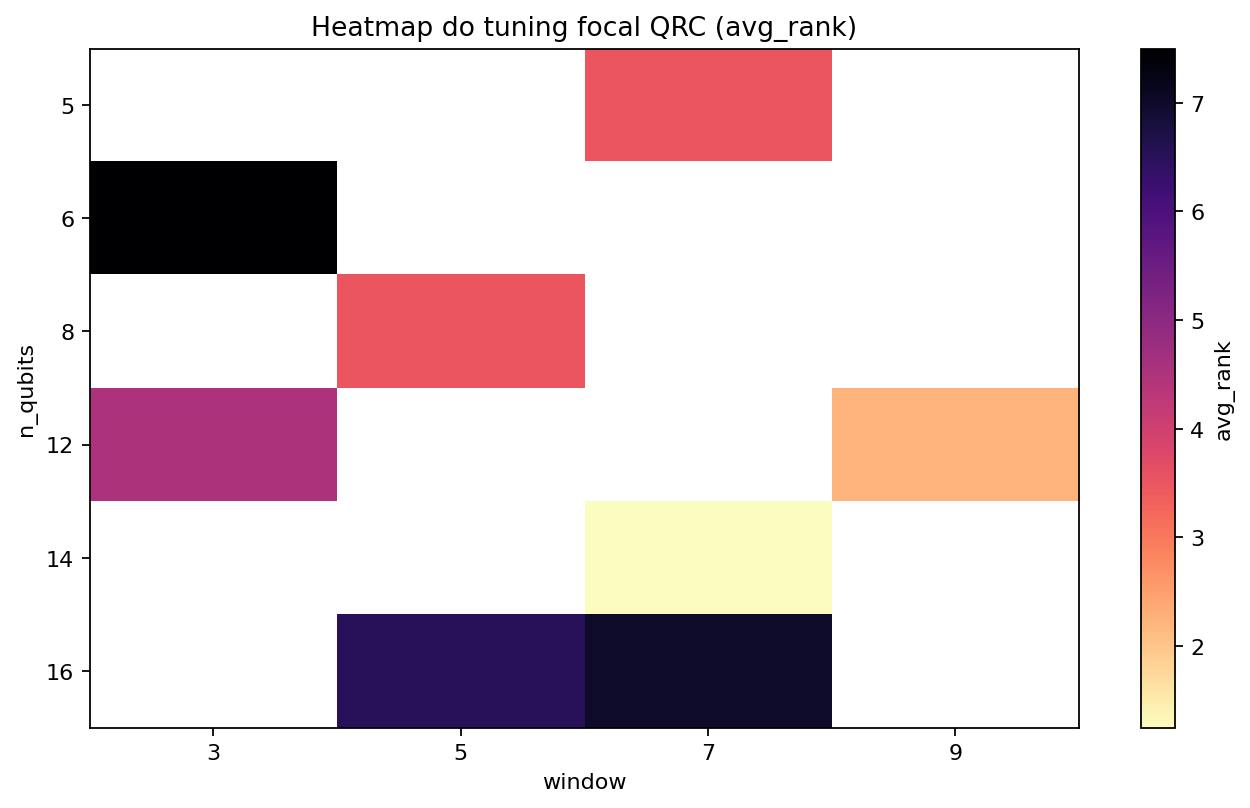
\includegraphics[keepaspectratio,alt={Mapa de calor do tuning de qubits e window para o QRC.}]{computational_results_20260402_222902/qrc_tuning_heatmap.png}}

A tabela mostra uma licao decisiva: aumentar \texttt{n\_qubits} e \texttt{window} nao melhora automaticamente o desempenho. O melhor ponto robusto ficou em \texttt{14x7}, enquanto \texttt{16x5} e \texttt{16x7} pioraram o rank medio.

\subsection{7. Uma funcao objetivo para escolher configuracoes comparaveis}\label{7-uma-funcao-objetivo-para-escolher-configuracoes-comparaveis}

O projeto nao ficou preso a um unico criterio. Alem do rank medio multi-metrica, foi proposta uma funcao objetivo escalar

\[
J(q, w) = G(q, w) \cdot C(q, w),
\]

com

\[
G(q, w) = \exp\left(\sum_k \omega_k \log\frac{m_k(q, w)}{r_k}\right),
\]

e

\[
C(q, w) = 1 + \lambda \, \frac{\mathrm{norm}(q) + \mathrm{norm}(w)}{2}.
\]

Aqui:

\begin{itemize}
\tightlist
\item
  \(m_k(q, w)\) sao as metricas do QRC;
\item
  \(r_k\) sao as metricas da melhor referencia nao-QRC;
\item
  \(\omega_k\) sao pesos por metrica;
\item
  \(\lambda = 0.05\) penaliza complexidade adicional.
\end{itemize}

Os pesos usados foram:

\begin{itemize}
\tightlist
\item
  \texttt{MAE\ =\ 0.3}
\item
  \texttt{RMSE\ =\ 0.3}
\item
  \texttt{WAPE\ =\ 0.2}
\item
  \texttt{sMAPE\ =\ 0.2}
\end{itemize}

O resumo da selecao ficou assim:

\begin{longtable}[]{@{}lll@{}}
\toprule\noalign{}
Criterio & Melhor configuracao & Valor \\
\midrule\noalign{}
\endhead
\bottomrule\noalign{}
\endlastfoot
Melhor rank medio multi-metrica & 14x7 & 1.25 \\
Melhor funcao objetivo escalar & 8x5 & 2.0030 \\
\end{longtable}

O criterio multi-metrica favorece \texttt{14x7}. A funcao objetivo penalizada favorece \texttt{8x5}.

\subsection{8. O que se ganha e o que se perde na ponte para QRC}\label{8-o-que-se-ganha-e-o-que-se-perde-na-ponte-para-qrc}

\subsubsection{8.1 O que se ganha}\label{81-o-que-se-ganha}

\begin{itemize}
\tightlist
\item
  uma nova classe de dinamica para representar series temporais;
\item
  uma formulacao muito natural para discutir observaveis e mistura de estados;
\item
  uma extensao conceitual elegante do paradigma de reservatorio.
\end{itemize}

\subsubsection{8.2 O que se perde}\label{82-o-que-se-perde}

\begin{itemize}
\tightlist
\item
  simplicidade operacional em relacao ao RC classico;
\item
  custo computacional, especialmente quando \texttt{qubits} e \texttt{window} crescem;
\item
  interpretabilidade imediata do estado interno.
\end{itemize}

\subsection{9. Por que o benchmark anterior precisa ser herdado}\label{9-por-que-o-benchmark-anterior-precisa-ser-herdado}

O QRC so faz sentido pedagogico neste projeto porque herda o benchmark do artigo 5. Sem esse benchmark, seria facil tratar o QRC como curiosidade isolada. Com ele, o leitor entende exatamente contra o que o QRC precisa ser comparado:

\begin{itemize}
\tightlist
\item
  \texttt{ETS}
\item
  \texttt{XGBoost}
\item
  \texttt{Prophet}
\item
  \texttt{Seasonal\ Naive}
\item
  \texttt{RC}
\item
  \texttt{LSTM}
\end{itemize}

Essa heranca metodologica e o que impede a fase quantica de perder contato com o problema de negocio.

\subsection{10. Conclusao}\label{10-conclusao}

A ponte entre RC classico e QRC esta pronta. O leitor agora tem um mapa formal, implementacional e experimental do salto para o quantico. O artigo final vai aproveitar exatamente essa ponte para executar e interpretar o QRC no recorte do Favorita, comparando \texttt{14x7}, \texttt{8x5} e os melhores modelos classicos.

\subsection{Entregaveis associados no repositorio}\label{entregaveis-associados-no-repositorio}

\begin{itemize}
\tightlist
\item
  implementacao do QRC: \texttt{code/qrc/model.py}
\item
  funcao objetivo: \texttt{code/qrc/objective.py}
\item
  documentacao da funcao objetivo: \texttt{code/qrc/OBJECTIVE.md}
\item
  artefatos deste artigo: \texttt{computational\_results\_20260402\_222902/}
\end{itemize}

\subsection{Referencias}\label{referencias}

\begin{itemize}
\tightlist
\item
  Fujii, K.; Nakajima, K. Harnessing disordered-ensemble quantum dynamics for machine learning.
\item
  Ghosh, S. et al. Quantum reservoir processing.
\item
  Qiskit documentation.
\item
  Monzani, F.; Ricci, E.; Nigro, L.; Prati, E. QRC-Lab: An Educational Toolbox for Quantum Reservoir Computing. arXiv:2602.03522.
\end{itemize}

        \end{document}
